\documentclass[headings=standardclasses,parskip=half]{scrartcl}

\usepackage[french]{babel}
\usepackage[margin=3cm]{geometry}
\usepackage{graphicx}
\usepackage[hidelinks]{hyperref}

\titlehead{
    \begin{center}
        
\includegraphics[width=5cm]{n7.png}
    \end{center}
}
\subject{Projet Données Réparties}
\title{Rapport}
\subtitle{}
\author{Enzo PETIT \and Nam VU}
\date{16 janvier 2022}
\publishers{ENSEEIHT – 2SN-A}


\begin{document}

\maketitle

\newpage

\tableofcontents

\newpage

\section{Introduction}

Le projet Linda a pour but de réaliser un espace partagé de données
typées.

Une version à mémoire partagée avec gestion de callback a été réalisée
ainsi qu'une version client-serveur en RMI se reposant sur cette dernière.

Pour la première version, la classe \texttt{linda.shm.CentralizedLinda}
a ainsi été complétée et des tests unitaires sous
\href{https://junit.org/junit5/}{JUnit 5}
ont été rédigés dans \texttt{linda.test.CentralizedLindaTest}.

La version client-serveur se trouve quand à elle dans le package
\texttt{linda.server} et utilise la version \textit{shm} inchangée pour
la partie serveur.

Enfin quelques applications utilisant Linda ont été réalisées
telle que la recherche de nombre premiers selon l'algorithme du
crible d'Erathosthène, en séquentiel et parallèle, ainsi que la
parallèlisation de l'application de recherche.

\section{Version en mémoire partagée}

\textit{Cette section reprend le rapport provisoire de décembre dernier.}

\subsection{Réalisation}

A l'instanciation, \texttt{CentralizedLinda} initialise trois tableaux
pour le stockage des tuples (\texttt{tupleSpace}) et les events
\emph{take} (\texttt{takeEvents}) et \emph{read} (\texttt{readEvents}).

Ces tableaux sont de type \texttt{CopyOnWriteArrayList} qui est une
variante \emph{thread-safe} de l'\texttt{ArrayList} classique adaptée
à un contexte concurrent où le nombre de lectures est bien supérieure
au nombre d'écritures.

Suivent après les détails d'implémentation des différentes opérations,
plus ou moins dans l'ordre de réalisation :

\subsubsection{\texttt{tryTake}, \texttt{tryRead}}

Ces deux méthodes sont non bloquantes, on itère simplement sur la liste
(en partant de la tête) et on renvoie le premier tuple (le plus vieux)
qui match le template. \texttt{null} est renvoyé si aucun tuple
actuellement stocké ne correspond.

\subsubsection{\texttt{takeAll}, \texttt{readAll}}

Même chose que précedemment mais on stocke tous les tuples correspondants
dans une \texttt{ArrayList} que l'on renvoie à la fin (qui est vide
si aucun résultat).

\subsubsection{\texttt{eventRegister}}

En commençant à vouloir implémenter les \texttt{take} et \texttt{read}
bloquant on s'est demandé comment pouvait-on \textit{proprement} et avec le
moins d'effort possible bloquer et débloquer les appels : le principe
des event nous a paru bien adapté pour réaliser cette tâche
(détails plus loin).

En mode \texttt{IMMEDIATE} un tuple est retourné immédiatement dans
le callback en cas de match sur l'espace actuel
(via \texttt{tryTake}/\texttt{tryRead}),
sinon on range l'event en attente dans le tableau correspondant
(\texttt{takeEvents} ou \texttt{readEvents}).

Le callback est transformé en amont en \texttt{AsynchronousCallback}
afin d'éviter les problèmes liés au blocage du thread principal ou
d'enregistrements récursifs de callbacks.

\subsubsection{\texttt{write}}

La méthode \texttt{write} étant la \textit{porte d'entrée} de tous les tuples
vers l'espace de stockage de Linda, c'est là qu'on en profite pour
\textit{résoudre} les event en attente le cas échéant.

Ainsi on itère d'abord sur les \emph{read} en attente (\texttt{readEvents}),
vérifie si le tuple à écrire \textit{match} le template de l'event et le cas
échéant on appelle le callback correspondant.

Ensuite on fait de même avec les \emph{take} en attente (\texttt{takeEvents})
mais au premier match (du plus vieux), on résout le callback et on retourne,
immédiatement. Le tuple n'est pas enregistré et les \emph{take} en attente
dessus mais plus récents attendront le prochain tuple correspondant.

Finalement si aucun \emph{take} n'attendait le tuple, on le sauvegarde dans
\texttt{tupleSpace}.

Un tuple en entrée peut ainsi résoudre tous les \emph{read} en attente mais
qu'un seul \emph{take} en attente, le plus vieux.

\subsubsection{\texttt{take}, \texttt{read}}

Un \emph{take} ou \emph{read} bloquant revient à enregistrer un event
\emph{immédiat} dont le callback renvoie le tuple passé en entrée,
rester bloqué jusqu'à résolution de celui-ci et finalement renvoyer
son résultat.

On utilise pour faire ça une \texttt{LinkedBlockingQueue}, queue bloquante :
le callback de l'event correspond à la méthode \texttt{offer} de la queue
(dépôt non bloquant) qui sera éventuellement appelée lors d'un \emph{write}.

Le \texttt{take}/\texttt{read} reste lui bloqué sur le \texttt{take} de la
queue et renverra son résultat quand il sera débloqué par un dépôt dans
la queue.

\subsection{Tests}

Tous les tests \texttt{Basic} fournis passent en l'état.

Une classe de tests unitaires \href{https://junit.org/junit5/}{JUnit 5}
\texttt{linda.test.CentralizedLindaTest} a aussi été écrite.

\begin{figure}[h]
    \centering
    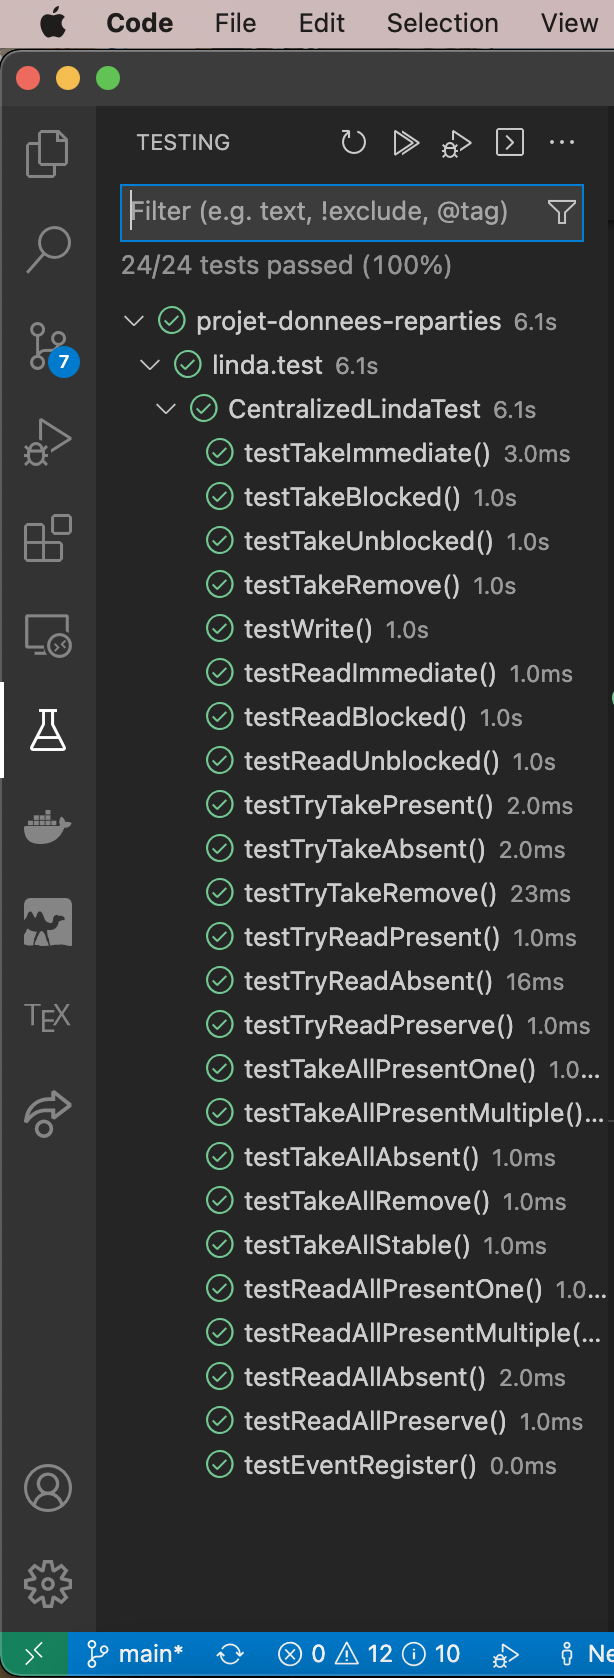
\includegraphics[scale=0.5]{tests-results.png}
    \caption{Résultats des tests définis dans
        \texttt{linda.test.CentralizedLindaTest}\\
        (Visual Studio Code + Extension Pack for Java)}
\end{figure}

\section{Version client / mono-serveur}

\textit{Package \texttt{linda.server}}

\subsection{Serveur}

Une interface \texttt{LindaServer} a été définie, étandant \texttt{Remote},
et reprend les méthodes définies dans l'interface \texttt{Linda} à la
différence que toutes les méthodes \texttt{throws RemoteException} et
que \texttt{eventRegister} prend en paramètre un \texttt{eventRegister}.

\texttt{eventRegister} est une interface qui étand aussi \texttt{Remote}
et représente un callback à exécuter sur le client.

L'implémentation de \texttt{LindaServer} est rédigée dans
\texttt{LindaServerImpl}. Cette classe initialise un noyau Linda en
mémoire partagée et transmets directement tous les appels distants au
noyau à l'exception du \texttt{eventRegister} : pour cette méthode,
on transmet au kernel un callback local qui résoudra le callback distant.
Ainsi tout est transparant pour le noyau en mémoire partagée.

\subsection{Client}

De la même manière \texttt{LindaClient} récupère un \texttt{LindaServer}
en RMI puis fonctionne de manière transparente pour les appplications en
local en ne faisant que transferer directement toutes les requêtes au
serveur distant.

Exception est encore faite pour \texttt{eventRegister} qui est un peu plus
complexe: on envoie au serveur un \texttt{RemoteCallback} via
\texttt{RemoteCallbackAdapter} qui s'occupera de répondre au callback
local côté client.

\section{Applications}

\subsection{Calcul des nombres premiers}

\textit{Package \texttt{linda.primes}}

\subsubsection{Séquentiel}

La classe \texttt{Sequential} implémente une version sequentielle basique
du crible d'Erathosthène en utilisant Linda.
On parcours les nombres de 2 à \(n\) : si il n'est pas présent dans Linda
(par \texttt{tryRead}) alors le nombre est premier et on rajoute tous
ses multiples dans Linda.

\subsubsection{Parallèle}

On fournit dans \texttt{Parallel} une tentative de parallèlisation de
cet algorithme peu parallèlisable.

On commence par enregistrer dans Linda tous les nombres en les marquant
premiers (initialisation du crible).

Autant de \texttt{Worker}s que de nombres sont ensuite créés : ils
s'occupent de retirer leurs multiples de Linda et abandonnent leur
tâche si leur nombre de départ s'avère non premier (retiré par un autre
\texttt{Worker}).
Tous ces \texttt{Worker}s sont exécutés dans des
threads grâce à un \texttt{ExecutorService} initialisé par
\texttt{Executors.newWorkStealingPool}.

Enfin, dans le thread principal on se bloque jusqu'à
l'éxecution complète de tous les \texttt{Worker}s.

\texttt{Résultats}

En testant la recherche jusqu'à 10000 il est clair que la parallèlisation
du crible d'Erathosthène est peu efficace. On obtient un temps de traitement
triple par rapport à la version séquentielle qui s'explique par l'overhead
généré par la création de threads et la répétitions d'opérations : ne pouvant
savoir si un nombre et premier dès le départ, on commence malgré tout
à marquer ses multiples.
Aussi notre implémentation de Linda fait que les lectures sont peu efficaces
car on itère sur toute la liste à chaque accès.

\subsection{Recherche approximative dans un fichier}

\textit{Package \texttt{linda.search.evolution}}

Cette application recherche dans un fichier de mots celui qui est le plus \textit{proche} du mot donné en entrée.

Une base de l'application était déjà faite, mais celle-ci devait être étendue avec d'autres fonctionnalités.

Pour chaque nouvelle fonctionnalité, une explication de l'implémentation se trouve dans ce qui suit.

\subsubsection{Simultanéité des chercheurs}

On voulait permettre à l'application d'autoriser plusieurs chercheurs en simultané sur une même requête.
Cela a été fait en modifiant plusieurs choses.

\begin{figure}[h]
    \centering
    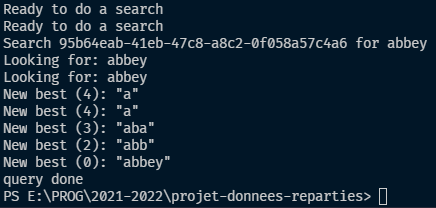
\includegraphics[scale=0.5]{plusieurs-chercheurs.png}
    \caption{Exemple d'exécution avec plusieurs chercheurs sur la même requête
        - 'abbey' dans un dictionnaire anglais}
\end{figure}

Tout d'abord, le tuple de requête contient un nouveau paramètre : le nombre de chercheurs ayant pris la recherche en charge.
Le manager initialise ce paramètre à 0.

Ensuite, quand un chercheur trouve un tel tuple, il le prend, regarde si il reste de la place pour d'autre chercheurs sur cette recherche,
et le redépose avec une valeur mise à jour dans l'espace le cas échéant.
Dans tous les cas, le chercheur va ensuite travailler normalement, mais au lieu de notifier la fin de son travail, il notifie qu'il
est toujours opérationnel.

Enfin, le manager va effectuer une attente semi-active pour savoir si il reste encore des chercheurs affectés à sa requête.
Quand il n'y en a plus, on considère la recherche comme terminée.

Le choix de l'attente active a été faite dans le cas où le chercheur viendrait à \textit{planter}, car la consigne spécifiait un
\textit{arrêt arbitraire de chercheurs}, que nous avons interprété en tant que tel. Dans ce cas, toute sorte
de notification de fin de travail est impossible.

Si cela n'était pas ce qui était désiré, nous avons pris l'autre partie pour la rétraction d'un manager
(voir la partie concernée ci-dessous).

\begin{figure}[h]
    \centering
    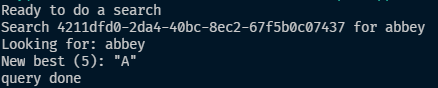
\includegraphics[scale=0.5]{arret-chercheurs.png}
    \caption{Exemple d'exécution avec arrêt prématuré des \texttt{Searcher}s -
        Le \texttt{manager} détecte l'absence de chercheur restants et termine}
\end{figure}

\subsubsection{Simultanéité des managers}

L'on souhaitait ici avoir plusieurs managers déposant des requêtes différentes.

La simple solution pour permettre cela était de marquer les données avec l'UUID de la requête.

Il fallait également attendre la prise en charge de la recherche par un des chercheurs avant
de considérer la fin de celle-ci.

\begin{figure}[h]
    \centering
    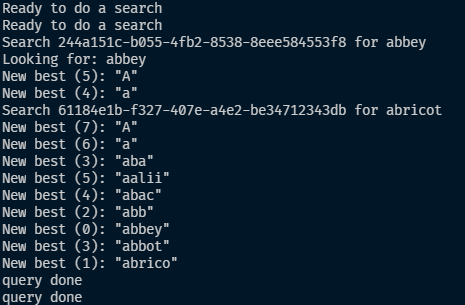
\includegraphics[scale=0.5]{plusieurs-managers.png}
    \caption{Exemple d'exécution avec 2 \texttt{Searcher}s
        et 2 \texttt{Manager}s - 'abbey' (présent) et 'abricot' (absent)}
\end{figure}

\subsubsection{Linda version serveur}

Ici, rien n'est à modifier, le code marchait à la perfection en étant simplement transposé,
même si les managers et les chercheurs sont dans des clients différents.

\subsubsection{Retrait de managers}

En contraste avec la vision prise pour les chercheurs, on considère ici que les managers se \textit{retirent}
moins brusquement.

Au lieu de faire une attente active du côté des chercheurs, on décide alors la présence dans
l'espace linda d'une variable \textit{de garde} que l'on retire quand on souhaite interrompre la recherche.

Pour permettre d'indiquer un temps d'attente maximum, l'on surcharge le constructeur avec un nouveau
paramètre.

On peut alors déclarer un objet partagé et attendre un temps maximal à l'aide de la fonction \texttt{wait()},
et reprendre l'exécution plus tôt à l'aide de la fonction associée \texttt{notify()}.

De plus, si un chercheur est interrompu dans sa recherche, il est réinitialisé et attend une nouvelle
requête.

\end{document}
